\chapter{Mechanical Design and URDF Modeling of the Hand Exoskeleton}
\section{Overview of the Design Pipeline}
This chapter describes the mechanical design and modeling process adopted for the development of the hand exoskeleton, focusing on the creation of a consistent and simulation-ready representation of the system. The objective is to show how the components were created, assembled and then used in the ROS2 environment to recreate the kinematics and dynamics of the case-study exoskeleton.

The exoskeleton's design was already studied and realized by Eng. Bartalucci in his thesis work, \textit{A Kinaesthetic Hand Exoskeleton System Toward Robot-augmented Rehabilitation Therapies in the Health 4.0 era} \cite{Bartalucci2024_Exoskeleton}, which this thesis stems from. From some measurements presented on Bartalucci's work, it was possible to deduct the dimensions of every component with an estimated error in the order of hundredths of a centimeter ($\sim10^{-4}m$). 


Following the mechanical design phase, the CAD models are translated into a URDF description. This step involves the definition of links, joints, reference frames, and their hierarchical relationships, enabling the representation of the exoskeleton as a kinematic tree suitable for simulation and control. Of the outmost importance was a Fusion360's plug-in, \textbf{ACDC4Robot} \cite{ACDC4Robot}, that automatically created the URDF once the components were assembled into the exoskeleton. Even if some modifications were necessary to make this URDF work, this plug-in simplified a lot the work's pipeline.

Once the URDF is functional, it's possible to use it in the ROS2 environment and verify if the dimensional and inertial properties are realistic.

\section{CAD Modeling of the Exoskeleton Components}
The exoskeleton components were modeled using \textbf{Fusion 360}, adopting a parametric and modular design approach. This choice facilitates iterative refinements and allows individual parts to be modified without affecting the overall assembly. As previously said, each component was designed with reference to dimensions derived from Bartalucci's thesis \cite{Bartalucci2024_Exoskeleton}.

In the reference design presented in Bartalucci's thesis \cite{Bartalucci2024_Exoskeleton}, the hand exoskeleton is structured as a set of \textbf{finger modules}, each corresponding to a single finger. The overall mechanical architecture is shared among the modules, while the primary differences are related to their geometric dimensions, which are adapted to match the anatomical proportions of each finger. In this context, the adoption of a parametric CAD environment proved particularly effective, as it allowed the same design template to be reused and scaled across different finger modules by modifying a limited set of parameters, while preserving the overall mechanical consistency of the system.

The complete CAD assembly was analyzed using the set of verification tools available in Fusion 360, which provide built-in functionalities for assessing the mechanical consistency of the design. These tools were used to inspect joint alignments and  evaluate relative motion between components. The availability of interactive assembly constraints and motion visualization allowed the design to be iteratively refined, ensuring that joint placements and links' dimensions were compatible with the intended range of motion of the exoskeleton.

As a representative example of the proposed design methodology, the following section illustrates the modeling process of the index finger module. The geometric dimensions of this module are derived from the reference model presented in Bartalucci's thesis \cite{Bartalucci2024_Exoskeleton}, in which the hand exoskeleton is parameterized according to anatomical measurements. In particular, Bartalucci provides a set of reference points and corresponding distances for each finger, summarized in a dedicated table. From this table, the distance between two selected points relevant to the index finger mechanism is extracted and used as a design constraint for the corresponding CAD component.

\begin{figure}[ht]
  \begin{minipage}[b]{0.59\textwidth}
    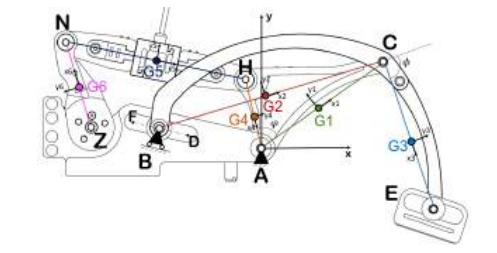
\includegraphics[width=\textwidth]{images/chapter1/progetto_riferimento.png}
    \caption{Lateral view of the FM mechanism}
  \end{minipage}
  \hfill
  \begin{minipage}[b]{0.4\textwidth}
    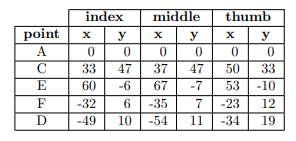
\includegraphics[width=\textwidth]{images/chapter1/tabella_riferimento.png}
    \caption{The optimized geometric dimensions of the FMs in mm}
  \end{minipage}
\end{figure}
\FloatBarrier

The figures and table shown above are reproduced from Bartalucci's thesis \cite{Bartalucci2024_Exoskeleton}, specifically Fig. 3.9 and Table 3.2, respectively. Starting from these reference dimensions, the index finger component was modeled in Fusion 360 by explicitly enforcing the same geometric distance between the corresponding points of the CAD model.

A straightforward approach to model the exoskeleton components consists in importing the lateral view of the finger module into Fusion 360 and scaling it using a reference measurement from the table, such as the length of segment AC. Once properly scaled, the individual components can be created directly from this reference geometry, and their dimensions can be subsequently verified against the remaining measurements reported in the table.

\begin{figure}[ht]
    \centering
    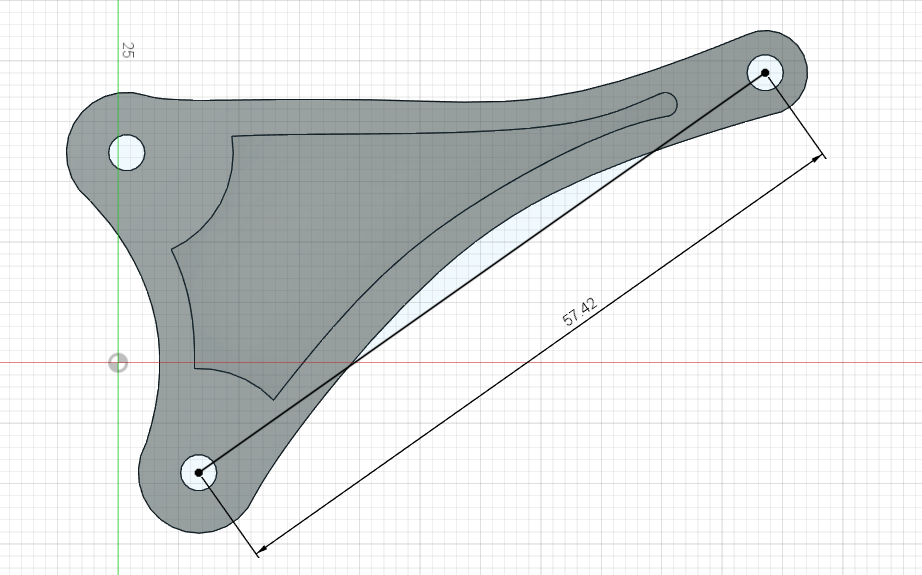
\includegraphics[scale=0.40]{images/chapter1/immagine_disegno.png}
    \caption{Component "Link AC", showing AC distance in mm}

\end{figure}
\FloatBarrier

From the reference coordinates reported in Table 3.2 of Bartalucci's thesis \cite{Bartalucci2024_Exoskeleton}, the length of segment AC was computed, resulting in a value of 57.4282 mm. The same distance was independently measured on the corresponding CAD model within the Fusion 360 environment, yielding an identical value of 57.42 mm, as shown in Figure 1.3. The resulting discrepancy is negligible and can be attributed to numerical rounding, confirming the geometric consistency between the reference data and the implemented CAD model. The same validation procedure was applied to all the remaining components of the finger module, obtaining the same positive results.

Once all components were modeled, the assembly was constructed using appropriate joints and validated through additional simulations. These simulations verified that the exoskeleton's end-effector exhibited realistic motion, consistent with the description in Bartalucci's thesis, based on the actuated revolute joint along the Z-axis, as illustrated in Figure 1.1.

\begin{figure}[ht]
    \centering
    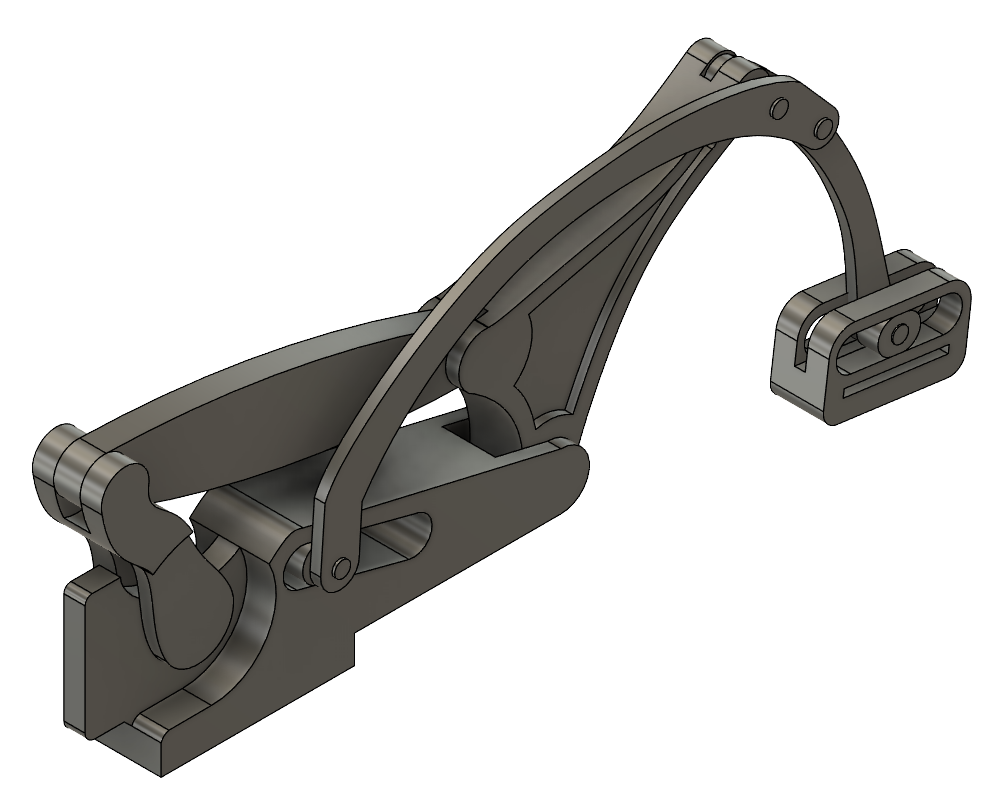
\includegraphics[scale=0.4]{images/chapter1/assemblato.png}
    \caption{Working assembly model of the exoskeleton designed in Fusion 360}
\end{figure}
\FloatBarrier


\section{URDF File from the CAD Model}
Once the mechanical design of the exoskeleton components was completed and validated in the CAD environment, the next step consisted in generating a \textbf{URDF} (Unified Robot Description Format) representation of the system. The URDF model provides a standardized description of the robot structure and represents the interface between the mechanical design and the simulation, kinematic, and control frameworks adopted in this work.

The conversion from the CAD assembly to the URDF format required the definition of a consistent link–joint hierarchy and the assignment of reference frames and geometric transformations to each component. This process was carried out while preserving the geometric consistency verified in the CAD environment and adapting the mechanical structure to the tree-based representation required by URDF.

To streamline this process, the \textbf{ACDCRobot} plug-in \cite{ACDC4Robot} was employed to automatically generate an initial URDF model directly from the Fusion 360 assembly. The plug-in exports the geometric meshes, defines the link structure, and computes the relative transformations between components, significantly reducing the manual effort required to obtain a first simulation-ready description of the system.

The URDF model generated through ACDCRobot provided a consistent initial representation of the exoskeleton, including the main links and joints of the mechanism. Nevertheless, additional refinement steps were required to ensure full compatibility with simulation and control tools. These refinements included numerical adjustments, the definition of joint limits, and the handling of the closed kinematic chains present in the original mechanical design.

The hand exoskeleton mechanism inherently includes multiple \textbf{closed kinematic chains}, resulting from the coupling of links required to reproduce human finger motion. Since URDF represents robotic systems as tree-structured kinematic graphs, such closed-loop mechanisms cannot be directly modeled and are therefore not supported by standard ROS-based kinematic and dynamic tools.

To address this limitation, the closed kinematic chains were deliberately \textbf{opened} at selected revolute joints, transforming the mechanism into an equivalent kinematic tree compatible with the URDF format. The opening points were chosen to preserve the physical meaning of the original design while minimizing their impact on the overall kinematic behavior.

\begin{figure}[ht]
    \centering
    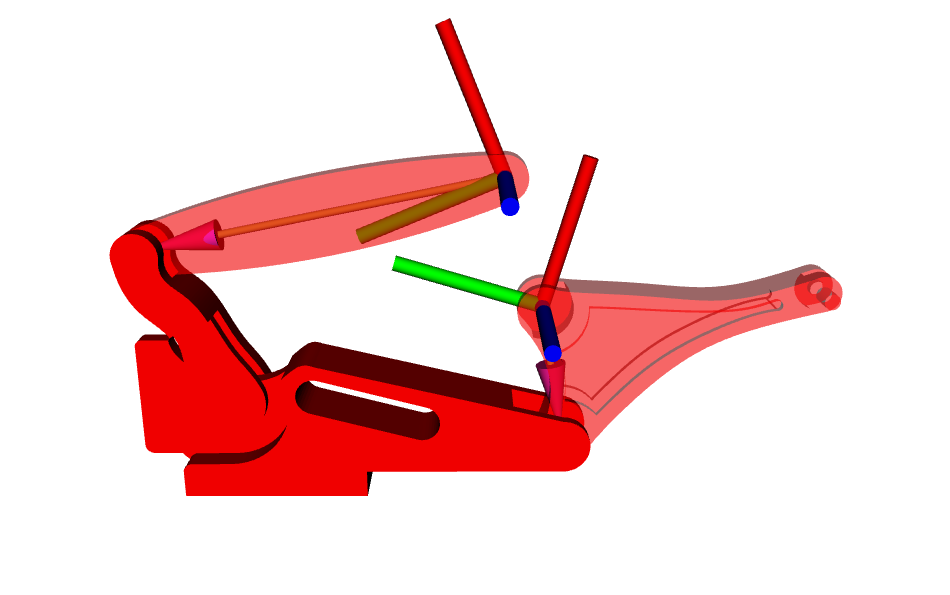
\includegraphics[scale=0.4]{images/chapter1/open_chain.png}
    \caption{Example of an opened kinematic chain in the exoskeletron's URDF model}
\end{figure}
\FloatBarrier

An illustrative example of this procedure is shown in figure above, which depicts one of the opened chains connecting the \textit{connecting rod} to \textit{link AC}. In the original mechanism, this connection forms part of a closed loop, while in the URDF representation it is split into two branches terminating in the auxiliary reference frames shown in the figure.

The geometric closure of the mechanism is not enforced at the URDF level but is instead restored within the software architecture by requiring the coincidence of the auxiliary frames associated with the opened chain. This condition is imposed during kinematic and dynamic computations through a constraint-based formulation implemented in a dedicated ROS node. In this way, the original closed-chain behavior of the mechanism is recovered while maintaining full compatibility with standard URDF and ROS tools.

The refined URDF model obtained through this process provides a robust foundation for the kinematic and dynamic modeling presented in the following chapters, where the imposed constraints are explicitly handled within the control and simulation framework.
